\chapter{CNN Compiling and Computation}
\label{chapter:CNNVersat}

\quad In section~\ref{section:darknet}, Neural Network Frameworks are introduced. This chapter is divided into two sections.
 Section~\ref{section:toolflow} is an overview of Toolflows that map Convolutional
Neural Networks using said frameworks into FPGA. Section~\ref{section:autotuning} introduces concepts to accelerating CNNs into 
deployed hardware like CGRAs.


%PAPERS
%https://www.cv-foundation.org/openaccess/content_cvpr_workshops_2014/W17/html/Gokhale_A_240_G-opss_2014_CVPR_paper.html
%

\section{Toolflows for Mapping CNNs in FPGAs}
\label{section:toolflow}

\quad Several software frameworks have been developed to accelerate development and high-performance execution of CNNs.
 Neural Networks Frameworks discussed in section~\ref{section:darknet} provide high level APIs together with high performance execution on Multi Core CPUs, GPUs, Digital Signal Processors (DSP) and Neural Processing Units (NPU)~\cite{smartphones}.
FPGAs provide an alternative to these architectures by being high-performance while also being low-power that can meet several requirements
like throughput and latency in diverse applications. Thus, toolflows that map descriptions of CNN into hardware architecture to perform inference of the Network
were created. Several toolflows and their interfaces are present in table~\ref{table:toolflow}.

\begin{table}[!htpb]
    \centering
    \begin{tabular}{lll}
    \hline
    \textbf{Toolflow Name} & \textbf{Interface}       & \textbf{Year}  \\ \hline
    fpgaConvNet            & Caffe \& Torch           & May 2016       \\
    DeepBurning            & Caffe                    & June 2016      \\
    Angel-Eye              & Caffe                    & July 2016      \\
    ALAMO                  & Caffe                    & August 2016    \\
    Haddoc2                & Caffe                    & September 2016 \\
    DNNWeaver              & Caffe                    & October 2016   \\
    Caffeine               & Caffe                    & November 2016  \\
    AutoCodeGen            & Proprietary Input Format & December 2016  \\
    Finn                   & Theano                   & February 2017  \\
    FP-DNN                 & Tensorflow               & May 2017       \\
    Snowflake              & Torch                    & May 2017       \\
    SysArrayAccel          & C                        & June 2017      \\
    FFTCodeGen             & Proprietary Input Format & December 2017  \\ \hline
    \end{tabular}
    \label{table:toolflow}
    \caption{CNN to FPGA Toolflows, adapted from~\cite{misc:cnntofpga}}
\end{table}
\subsection{Supported Neural Network Models}

\quad These toolflows support the most common layers in CNNs discussed in chapter~\ref{chapter:cnn}. The acceleration target changes
depending on toolflow. fpgaConvNet~\cite{fpgaconvnet} focuses more on feature extraction while offering non accelerated support for Fully Connected layers
by casting them as Convolutional Layers with 1x1 kernels.

\subsection{Architecture \& Portability}

\begin{figure}[!htbp]
    \centering
    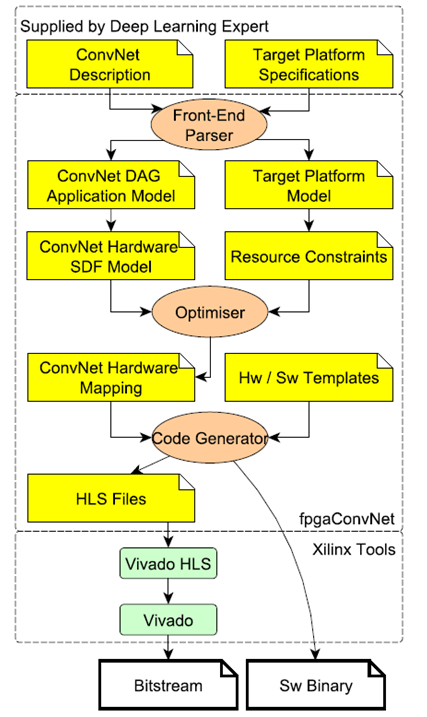
\includegraphics[width=0.5\textwidth]{Figures/fpgaconvnet.png}
    \caption{fpgaConvNet Architecture. Taken from~\cite{fpgaconvnet}}
    \label{figure:fpgaconvnet}
\end{figure}

As shown in figure~\ref{figure:fpgaconvnet}, fpaconvnet architecture consits of a Front-End Parser to capture
the number of layers to implement, their size and kernels. Then the architecture is optimized to the device target and Neural Network.
Finally, its mapped to hardware by using High Level Syntheses (HLS) which is a programming model for hardware based on C with a layer of abstraction.
\newpage
\section{CNN Auto Tuning Framework}
\label{section:autotuning}
